% ;; TeX-PDF-mode: t; TeX-master: "main" -*-%

%\documentclass[article,dr=phil,type=drfinal,colorback,accentcolor=tud9c]{tudthesis}
\documentclass[]{beamer}
 \usetheme{Madrid}
\usepackage{epigraph}
\usepackage{xspace}

\usepackage{import}
%\usepackage{enumitem}      % adjust spacing in enums
%\usepackage[colorlinks=true,allcolors=blue,breaklinks,draft=false]{hyperref}   % hyperlinks, includ
%\usepackage{ctable}
%\usepackage{footmisc}
\usepackage{hhline}


\usepackage{pgfplots}
\usepackage{booktabs}

\usepackage{colortbl}
\usepackage{color}

\usepackage{multicol}
\usepackage{multirow}
\usepackage{url}

\usepackage{listings}
\lstset{
  frame=Ltb,
  framerule=0pt,
  aboveskip=0mm,
  framextopmargin=0pt,
  framexbottommargin=0pt,
  framexleftmargin=0cm,
  framesep=0pt,
  rulesep=0pt,
  showstringspaces = false,
  basicstyle=\ttfamily,
  numbers=none,
  mathescape=true,
 % numbersep=-5pt,
 % numberstyle=\tiny,
 % numberfirstline=true,
 % firstnumber=auto,
  breaklines=true
}

\usepackage{tikz}
\usetikzlibrary{shapes}
\usetikzlibrary{arrows}
\usetikzlibrary{decorations.markings}
\usetikzlibrary{shapes.multipart}
\usetikzlibrary{shapes.arrows}
\usetikzlibrary{shapes.geometric}
\usetikzlibrary{positioning}
\usetikzlibrary{patterns}
\usetikzlibrary{calc,decorations.pathreplacing,matrix,shadows,fit,chains} 
\usetikzlibrary{trees,hobby,backgrounds}
\usepackage{tabularx,booktabs} 
\newcommand{\convexpath}[2]{
[   
    create hullnodes/.code={
        \global\edef\namelist{#1}
        \foreach [count=\counter] \nodename in \namelist {
            \global\edef\numberofnodes{\counter}
            \node at (\nodename) [draw=none,name=hullnode\counter] {};
        }
        \node at (hullnode\numberofnodes) [name=hullnode0,draw=none] {};
        \pgfmathtruncatemacro\lastnumber{\numberofnodes+1}
        \node at (hullnode1) [name=hullnode\lastnumber,draw=none] {};
    },
    create hullnodes
]
($(hullnode1)!#2!-90:(hullnode0)$)
\foreach [
    evaluate=\currentnode as \previousnode using \currentnode-1,
    evaluate=\currentnode as \nextnode using \currentnode+1
    ] \currentnode in {1,...,\numberofnodes} {
-- ($(hullnode\currentnode)!#2!-90:(hullnode\previousnode)$)
  let \p1 = ($(hullnode\currentnode)!#2!-90:(hullnode\previousnode) - (hullnode\currentnode)$),
    \n1 = {atan2(\y1,\x1)},
    \p2 = ($(hullnode\currentnode)!#2!90:(hullnode\nextnode) - (hullnode\currentnode)$),
    \n2 = {atan2(\y2,\x2)},
    \n{delta} = {-Mod(\n1-\n2,360)}
  in 
    {arc [start angle=\n1, delta angle=\n{delta}, radius=#2]}
}
-- cycle
}
% Define block styles  
\tikzstyle{materia}=[draw, text width=6.0em, text centered,
  minimum height=1.5em]

\tikzstyle{tpracticagray} = [materia,fill=gray!20, text width=10em, minimum width=8em,
  minimum height=3em, rounded corners, drop shadow]

\tikzstyle{nprocess} = [materia,fill=white, text width=4em, minimum width=4em,
  minimum height=3em]
\tikzstyle{oprocess} = [materia,fill=blue!20, text width=4em, minimum width=4em,
  minimum height=3em, rounded corners, drop shadow]


\tikzstyle{texto} = [above, text width=15em, text centered]
\tikzstyle{linepart} = [draw, thick, color=black!50, -latex', dashed]
\tikzstyle{line} = [draw, thick, -latex']

\newcommand{\practica}[2]{node (p#1) [practica]
  {\textit{#2}}}
\newcommand{\tpractica}[2]{node (p#1) [tpractica]
  {\textit{#2}}}
\newcommand{\tpracticagray}[2]{node (p#1) [tpracticagray]
  {\textit{#2}}}
\newcommand{\nprocess}[2]{node (p#1) [nprocess]
  {\textit{#2}}}
\newcommand{\oprocess}[2]{node (p#1) [oprocess]
  {\textit{#2}}}
\newcommand{\nprocessgray}[2]{node (p#1) [nprocessgray]
  {\textit{#2}}}

% Draw background
\newcommand{\background}[5]{%
  \begin{pgfonlayer}{background}
    % Left-top corner of the background rectangle
    \path (#1.west |- #2.north)+(-0.5,0.5) node (a1) {};
    % Right-bottom corner of the background rectanle
    \path (#3.east |- #4.south)+(+0.5,-0.25) node (a2) {};
    % Draw the background
    \path[fill=purple!10,rounded corners, draw=black!50, dashed]
      (a1) rectangle (a2);
    \path (a1.east |- a1.south)+(1.5,-0.4) node (u1)[texto]
      {\textit{#5}};
  \end{pgfonlayer}}

\newcommand{\backgroundNew}[5]{%
  \begin{pgfonlayer}{background}
    % Left-top corner of the background rectangle
    \path (#1.west |- #2.north)+(-0.5,0.5) node (a1) {};
    % Right-bottom corner of the background rectanle
    \path (#3.east |- #4.south)+(+0.5,-0.25) node (a2) {};
    % Draw the background
    \path[fill=orange!20,rounded corners, draw=black!50, dashed]
      (a1) rectangle (a2);
    \path (a1.east |- a1.south)+(2,-0.4) node (u1)[texto]
      {\textit{#5}};
\end{pgfonlayer}}

\newcommand{\backgroundgray}[5]{%
  \begin{pgfonlayer}{background}
    % Left-top corner of the background rectangle
    \path (#1.west |- #2.north)+(-0.5,0.5) node (a1) {};
    % Right-bottom corner of the background rectanle
    \path (#3.east |- #4.south)+(+0.5,-0.25) node (a2) {};
    % Draw the background
    \path[fill=gray!20,rounded corners, draw=black!50, dashed]
      (a1) rectangle (a2);
    \path (a1.east |- a1.south)+(2,-0.4) node (u1)[texto]
      {\textit{#5}};
\end{pgfonlayer}}

\colorlet{dblue}{blue!50!black}

\author{Antonio Flores Montoya}
\title{Datalog Disassembler}
\begin{document}
\maketitle


\begin{frame}
  \frametitle{What?}
  \begin{block}{}We want a dissassembler that generates \textbf{reassembleable} code
  \end{block}

  Given a binary, we need to determine:
  \begin{itemize}
  \item \textbf{Code Inference:} Which addresses correspond to instructions
    \begin{itemize}
    \item x86 instructions have variable sizes
    \item there are gaps between code blocks
    \end{itemize}
    \pause
  \item \textbf{Symbolization} Which data items should  be symbolic
    (addresses to other parts of  the program)
    \pause


    Example: {\color{dblue}\lstinline{mov RAX, 402020}}\\
    Is this an address or just an integer/float constant?

  \end{itemize}
  \pause
  These are hard problems, we want to
  \begin{itemize}
  \item try and combine different heuristics easily
  \item fast!
  \end{itemize}
  Could Datalog be the answer?
\end{frame}


\begin{frame}
  \frametitle{What is Datalog anyway?}

    Datalog is a declarative logic language 

  \begin{itemize}
  \item A subset of prolog (NOT turing complete but can be extended).
  \item Used for deductive databases
  \item Can express certain dataflow static analyses concisely
  \item Since recently, can generate efficient code\\
  \end{itemize}
\end{frame}


\begin{frame}
  \frametitle{Static Analysis with Datalog}
  Programs are encoded as facts
 
  \begin{tikzpicture}
    %\draw[help lines,step=.2] (0,0) grid (10,3);
    %\draw[help lines,line width=.6pt,step=1] (0,0) grid (10,3);
    %\foreach \x in {0,1,2,3,4,5,6,7,8,9,10}
    % \node[anchor=north] at (\x,0) {\x};
    %\foreach \y in {0,1,2,3}
    % \node[anchor=east] at (0,\y) {\y};
    \node [scale=0.9] (box) at (1,1) {
      \begin{minipage}{\textwidth}
        \begin{tabularx}{\textwidth}{lX}
          Instruction:&
        {\color{dblue}\lstinline{4000A0: mov RAX, 420020}}\\
        Becomes: &
        {\color{dblue}\lstinputlisting[aboveskip=0mm,belowskip=0mm]{instruction.dl}}\\
        \end{tabularx}
      \end{minipage}
     
    };
  \end{tikzpicture}
  \vspace{-0.5cm}
  
   \pause
   The analysis as inference rules
 
 \begin{tikzpicture}
%\draw[help lines,step=.2] (0,0) grid (10,3);
%\draw[help lines,line width=.6pt,step=1] (0,0) grid (10,3);
%\foreach \x in {0,1,2,3,4,5,6,7,8,9,10}
% \node[anchor=north] at (\x,0) {\x};
%\foreach \y in {0,1,2,3}
%    \node[anchor=east] at (0,\y) {\y};
\invisible{
\node  at (0,0) {};
}
\node [scale=0.85,anchor=south west] (box) at (2,0) { 
  \begin{minipage}{\textwidth}
    \vspace{0.5cm}
 {\color{dblue} \lstinputlisting{analysis.dl}}
\end{minipage}
};
\end{tikzpicture}
\end{frame}

\begin{frame}
  \frametitle{Prototype Architecture}
  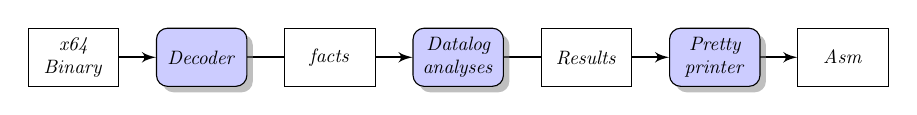
\begin{tikzpicture}[scale=0.7,transform shape]
    
    % Draw diagram elements
    \path \nprocess{0}{x64 Binary};
    \path (p0.east)+(1.5,0) \oprocess{1}{Decoder};
    \path (p1.east)+(1.5,0) \nprocess{2}{facts};
    \path (p2.east)+(1.5,0) \oprocess{3}{Datalog analyses};
    \path (p3.east)+(1.5,0)   \nprocess{4}{Results};
    \path (p4.east)+(1.5,0)   \oprocess{5}{Pretty printer};
    \path (p5.east)+(1.5,0)   \nprocess{6}{Asm};
    % Draw arrows between elements
    %% \path [line] (p1.west)+(-2,0)  -- node [above] {Binary} (p1);
    \begin{scope}[on background layer]
      \path [line] (p0) -- node [above] {} (p1);
      \path [line] (p1) -- node [above] {} (p3);
      % \path [line] (p2) -- node [above] {} (p3);
      \path [line] (p3) -- node [above] {} (p5);
      % \path [line] (p4) -- node [above] {} (p5);
      \path [line] (p5) -- node [above] {} (p6);
    \end{scope}


  \end{tikzpicture}
  \begin{description}
  \item[Decoder] Take the binary and generate facts:
    \begin{itemize}
    \item all the instructions at all possible offsets
    \item all data bytes in data sections
    \item symbols, relocations, etc.
    \end{itemize}
  \item[Datalog analyses] Use the datalog engine Souffle
    \begin{itemize}
    \item can generate C++ code
    \item has a decent profiler
    \end{itemize}
    
  \item[Pretty printer] Combine the results and print the assembler code
  \end{description}
\end{frame}


\begin{frame}{Datalog Analyses}

  \begin{itemize}
  \item \textbf{Code Inference:} Which addresses correspond to instructions
  \item \textbf{Symbolization:} Which data items should be symbolic
  \end{itemize}
\end{frame}    
\begin{frame}
  \frametitle{Code Inference}
  \begin{enumerate}
  \item Start from 'entry points' and traverse the code recursively
    
  \item Any immediate number that falls into the address range is considered as an entry point
    (plus all elements in data sections)
    \pause
    {\color{dblue}\lstinline{4000A0: mov RAX, 420020}}\\
    Assume 420020 is an entry point
    \pause
    \begin{block}{Implicit assumption}
      The addresses of all code blocks appear somewhere in the code, in the data,
      or they are addressed RIP-relative
    \end{block}
\pause
  \item Once finished, look for blocks whose addresses overlap\\
    (it can happen because we over-approximate the entry points)
  \item Solve the conflicts between blocks using heuristics
  \end{enumerate}
\end{frame}
\begin{frame}{Symbolization}
  \begin{block}{Naive approach}
    Everything that falls in the range of
    possible addresses is an address
    \end{block}
  \begin{itemize}
  \item False positives: Value collisions\\
    Consider additional criteria:
    \begin{itemize}
     \item the element is used as an address
     \item the element is not used as something else
    \end{itemize}
    Infer \textbf{data access patterns} using lightweight static analyses\\
    \alert{So far, all false positives are in the data sections}
  \item False negatives: Pointer reattribution\\
    \textbf{data access patterns} can be useful here too
  \end{itemize}
\end{frame}
\begin{frame}{Data Access Patterns}
  Examples:
  \begin{itemize}
  \item  {\color{dblue}\lstinline{mov RAX, WORD PTR 402020}}\\
    Content at 402020 is 16 bits long so it ``cannot'' be a pointer

  \item<2-> {\color{dblue}\lstinline{mov RAX, BYTE PTR [RAX*8+402020]}}\\
    Content at 402020 is 8 bits long  but possibly also at 402020+8, 402020+16...
    \visible<3->{ until when?}

  \item<5-> What about {\color{dblue}\lstinline!mov RAX, WORD PTR [RCX]!}?\\  
  \end{itemize}
  \visible<4->{
  Current approach:}
  \begin{itemize}
  \item<4-> Until we reach another data access
  \item<6> Use static analysis to estimate the \textbf{value of registers}
   \end{itemize}
     
\end{frame}
\begin{frame}{Register Value Analysis}
 Infer predicates of the form:

 {\center\color{dblue}\lstinline{value_reg(EA,Reg,EA1,Reg1,Multiplier,Offset)}
 \endcenter}

Which represent:

$$Reg@EA = (Reg1@EA1)* Multiplier + Offset$$
\pause
Example:
\begin{tabular}{ll}

  \multirow{2}{*}{{\color{dblue}\lstinputlisting[aboveskip=0mm,belowskip=0mm]{value_analysis.s}}}
  & value\_reg(1, RAX,0, None, 0, 40000)\\
  & value\_reg(2, RAX, 1, RAX, 1, 2)\\
  \\
  
  \visible<3>{And propagate: & value\_reg(2, RAX, 0, None, 0, 40002)}\\
\end{tabular}
    
\end{frame}

\begin{frame}{Symbolization}
  \begin{block}{Naive approach}
    Everything that falls in the range of
    possible addresses is an address
    \end{block}
  \begin{itemize}
  \item {\color{gray}
    False positives:
    Value collisions\\
    Consider additional criteria:
    \begin{itemize}
     \item \color{gray}the element is used as an address
     \item \color{gray}the element is not used as something else
    \end{itemize}
    Infer \textbf{data access patterns} using lightweight static analyses\\
   \invisible{ \alert{So far, all false positives are in the data sections}}}
  \item False negatives: Pointer reattribution\\
    \textbf{data access patterns} can be useful here too
  \end{itemize}
\end{frame}
\begin{frame}{Pointer Reattribution}
  \begin{tikzpicture}
    %\draw[help lines,step=.2] (0,0) grid (10,3);
    %\draw[help lines,line width=.6pt,step=1] (0,0) grid (10,3);
    %\foreach \x in {0,1,2,3,4,5,6,7,8,9,10}
    % \node[anchor=north] at (\x,0) {\x};
    %\foreach \y in {0,1,2,3}
    % \node[anchor=east] at (0,\y) {\y};
    \node[anchor=north west,scale=0.95]  (box) at (0,0) {
      \begin{minipage}{0.7\textwidth}
      {\color{dblue}\lstinputlisting[aboveskip=0mm,belowskip=0mm]{pointer_reattribution.s}}
      
      The immediate points outside the memory regions
     
      \visible<2->{
        But it should be treated as an symbolic address:\\

        {\color{dblue}\lstinline{ mov RCX, [RAX+L_610000+1000]}}
        }
      \end{minipage}
    };
    \node[anchor=north west] (box) at (8,0){
      \begin{tabular}{r|c|}
       \multicolumn{2}{c}{
        Address~~   Content}\\
    \cline{2-2}
    600000 & .bss \\ \cline{2-2}
           & \vdots \\ \cline{2-2}
    610000 & .bss \\ \cline{2-2}
    610001 & -  \\ \cline{2-2}
           & \vdots \\ \cline{2-2}
    611000 & -  \\ \cline{2-2}
  \end{tabular}
};
    \end{tikzpicture}
\end{frame}
\begin{frame}
  \frametitle{Experiments}
  \begin{itemize}
    \item
   Three compilers (versions): gcc 5.4, gcc 8, and clang 3.8
\item
  Five optimization flags: None, -O1, -O2, -O3 and -Os
  \item
    Three benchmarks: Coreutils, (a subset of) CGC, Real world examples
  \end{itemize}

  Funtionality tests
  \begin{tabular}{llllll}
    Benchmark       & Examples    & Combinations   & Succeed   & Failed  & \%\\ \hline
    Coreutils       & 106         & 1590           & 1590      &   0     & 100\% \\
    CGC             & 89          & 1335           & 1256      &  29\footnote{50 testing timeouts}    & 94\%    \\
    Real world      & 22          & 330            &  327      &   3     & 99\%     \\
  \end{tabular} 
\end{frame}

\begin{frame}
  \frametitle{Performance: Coreutils}
\center
\begin{tikzpicture}
\begin{axis}[
      xlabel=size (bytes),
      ylabel=time (seconds)]
\addplot+[
    only marks,
    scatter,
  %  mark=halfcircle*,
    mark size=2pt]
table[meta=time]
{coreutil_times.csv};
\end{axis}
\end{tikzpicture}
\end{frame}

\begin{frame}
  \frametitle{Performance: Real world examples}

\center
\begin{tikzpicture}
  \begin{axis}[
      xlabel=size (bytes),
      ylabel=time (seconds)]
   
    \addplot+[
%       nodes near coords,
%    point meta=explicit symbolic,
    only marks,
    scatter,
    %  mark=halfcircle*,
    mark size=2pt]
table[meta=time]{real_times.csv};
\end{axis}
\end{tikzpicture}
\end{frame}

\begin{frame}
  \frametitle{Performance: CGC}

\center
\begin{tikzpicture}
\begin{axis}[
      xlabel=size (bytes),
      ylabel=time (seconds)]
\addplot+[
    only marks,
    scatter,
  %  mark=halfcircle*,
    mark size=2pt]
table[meta=time]
{CGC_times.csv};
\end{axis}
\end{tikzpicture}
\end{frame}

\end{document}
